\chapter{粘性流体动力学基础}
\thispagestyle{empty}
\section{流体的粘性及其对流动的影响}
\subsection{流体的粘性}
由于流体粘性影响,均匀流经平板时,贴着平板表面的流体速度降为零,称为\red{流体与板面间 “无滑移” 边界条件}。由于收到内层流体的摩擦力、外层流体的速度有变慢趋势,反过来,由于收到外层流体的摩擦力,内层流体的速度有变快趋势。流层简单“互相牵扯”作用一层层向外传递,在距离板面一定距离后,这种作用逐步消失,速度分布变为均匀。

\defination[流体粘性]
{流层之间“阻碍”流体相对变形趋势的能力称为\dy[流体粘性]{LTNX},相对错动(剪切)流层间的一对摩擦力即\dy[粘性剪切力]{NXJQL}。}

\begin{figure}[!htb]
	\centering
	\begin{minipage}{0.45 \linewidth}
		\centering
		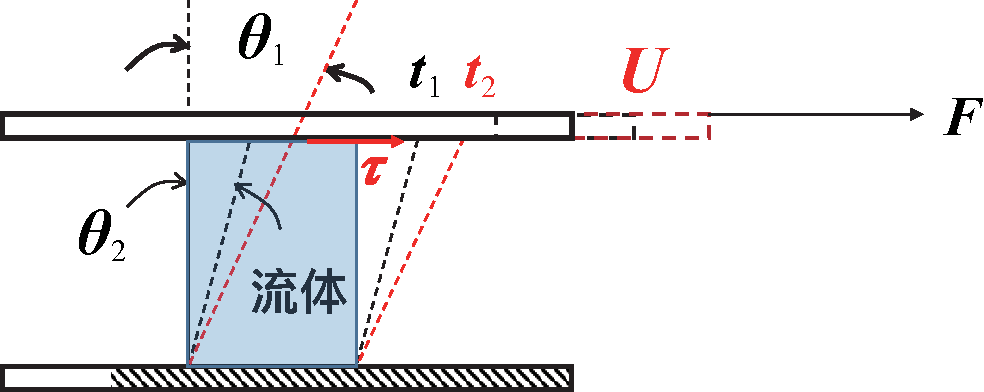
\includegraphics[width=\linewidth]{pic/流体粘性实验.pdf}
		\caption{流体剪切实验}
		\label{流体剪切实验2}
	\end{minipage}
	\begin{minipage}{0.45 \linewidth}
		\centering
		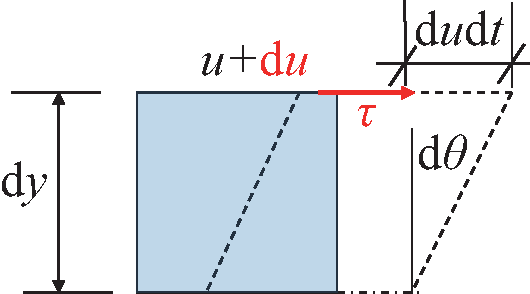
\includegraphics[width=0.7\linewidth]{pic/粘性几何关系.pdf}
		\vspace*{0.1em}
		\caption{流体剪切几何关系}
		\label{流体剪切几何关系2}
	\end{minipage}
\end{figure}
\vspace*{-1em}

如图\ref{流体剪切实验2}所示,可以得到剪切力和粘性剪切应力的表达式
\begin{equation}
	F = \mu \dfrac{U}{h}A, \qquad \tau = \dfrac{F}{A} = \mu \dfrac{U}{h}
\end{equation}

\theorem[牛顿粘性应力公式]
{
	\quad \vspace*{-1em}
	\begin{equation}
		\tau = \mu \dfrac{\d u}{\d y}
		\label{牛顿粘性应力公式2}
	\end{equation}
	其中,$\mu$是流体的粘性系数,$u$是流体的运动速度。\dy[牛顿粘性应力公式]{NDNXYLGS}表明粘性剪切应力不仅与速度梯度有关,而且与物性有关。
}
\noindent 从牛顿粘性应力公式可以看出:\vspace*{-0.5em}
\begin{itemize}
	\item 流体的剪应力与压强$p$无关。\vspace*{-0.5em}
	\item 当$\tau \neq 0$时,$\dfrac{\d u}{\d y} \neq 0$,即无论剪应力多小,只要存在剪应力,流体就会发生变形运动,呈现速度梯度。\vspace*{-0.5em}
	\item $\dfrac{\d u}{\d y}=0$时,$\tau = 0$,即只要流体静止或无变形,就不存在剪应力,流体不存在静摩擦力。
\end{itemize}
因此,\textbf{牛顿粘性应力公式可看成流体易流性的数学表达}。

如图\ref{流体剪切几何关系2}所示,可以找到几何关系
\begin{equation}
	\d \theta \d y = \d u \d t , \quad \dfrac{\d \theta }{\d t} = \dfrac{\d u}{\d y}
\end{equation}
即微团垂直线在单位时间内顺时针的转角$=$速度梯度,速度梯度也表示流体微团的\dy[剪切变形速度]{JQBXSD}或\dy[角变形率]{JBXL}。

一般地,流体剪切应力与速度梯度的关系表示为:
\begin{equation}
	\tau = A + B \left(\dfrac{\d u}{\d y}\right)^n
\end{equation}
但是我们一般只研究\dy[牛顿流体]{NDLT}(如水、空气、汽油、酒精等),即满足牛顿粘性应力公式\eqref{牛顿粘性应力公式2}的流体。

\warn[\textbf{液体和气体产生粘性的物理原因不同}\\
\hspace*{2em}液体的粘性主要来自于液体分子间的{\blue[内聚力]},气体的粘性主要来自于气体分子的{\blue[热运动]}。因此液体与气体{\red[动力粘性系数随温度变化的趋势相反]}(气体粘性系数随温度的升高而升高,液体粘性系数随温度的升高而降低),但动力粘性系数与压强基本无关。]

\defination[动力学粘性系数和运动学粘性系数]
{
	在许多空气动力学问题里,粘性力和惯性力同时存在,在式子中$\mu$和$\rho$往往以$\dfrac{\mu}{\rho}$的组合形式出现,用符号$\nu$表示:(注意$\mu$和$\nu$的物理区别)
	{
		\begin{itemize}
			\item \dy[动力学粘性系数]{DLXNXXS}:$\mu \quad \left[\dfrac{\text{N}\cdot \text{s}}{\text{m}^2}\right]\qquad \mu_{\text{a}} = 1.7894\times 10^{-5} \, \text{kg/m/s}, \quad \mu_{\text{w}} = 1.139 \times 10^{-3}\, \text{kg/m/s}$  
			
			\item \dy[运动学粘性系数]{YDXNXXS}:$\nu = \dfrac{\mu}{\rho} \quad \left[\dfrac{\text{m}^2}{\text{s}}\right]\qquad \nu_\text{a} = 1.461\times 10^{-5} \, \text{m}^2/\text{s} \quad \nu_\text{w} = 1.139\times 10^{-6} \, \text{m}^2/\text{s}$
		\end{itemize}
	}
}
可以看出:空气动力粘性不大,初步近似研究时可忽略其粘性作用,忽略粘性的流体称为\dy[理想流体]{LXLT}。
\vspace*{0.5em}

\noindent 流体粘性的特点总结如下:
\vspace*{-0.5em}
\begin{itemize}
	\item 流体的 剪切变形 是指流体质点之间出现相对运动 例如流体层间的相对运动、产生速度梯度;\vspace*{-0.5em}
	\item 流体的粘性是指流体抵抗剪切变形或质点之间的相对运动的能力,是流体的物理属性;\vspace*{-0.5em}
	\item 流体的粘性力是抵抗流体质点之间相对运动,例如流体层间的相对运动 的剪应力或内摩擦力;\vspace*{-0.5em}
	\item 在静止状态下流体不能承受剪切力;但是在运动状态下流体可以承受剪力,剪切力大小与流体速度梯度有关 而且与流体种类有关;\vspace*{-0.5em}
	\item 粘性流体在流动过程中必然要克服内摩擦力做功,因此流体粘性是流体发生机械能损失的根源 。
\end{itemize}

\subsection{粘性对流动的影响}
\noindent \textbf{1. 绕平板的直匀流}

































